\chapter{Einleitung}

\section{Einführung und Motivation}

Die BRUNATA-METRONA GmbH \& Co. KG zählt seit mehr als 50 Jahren zu den führenden Anbietern verbrauchsbasierter Abrechnungssysteme für Heiz- und Wasserkosten. Das Unternehmen hat seine Marktposition durch die schrittweise Erweiterung seines Dienstleistungsangebots und den gezielten Einsatz digitaler Tools gesichert. Diese strategische Ausrichtung half dabei, auch in komplexen Phasen der Branchenentwicklung wettbewerbsfähig zu bleiben.

Um die Effizienz weiter zu steigern und Dienstleistern bzw. Kunden neue Interaktionsmöglichkeiten zu bieten, evaluieren Abteilungen regelmäßig neue Technologien zur Integration in bestehende Abläufe. Hier stehen aktuell vor allem KI-gestützte Lösungen, wie die Implementierung eines Chatbots zur Unterstützung der Kundenkommunikation, und die Verwendung von \emph{Computer-Vision-Algorithmen} für die automatisierte Ablesung von Zählerständen im Fokus.

Letzteres stellt die Grundlage der \textit{Augmented Reality}-Technologie (AR) dar, die in den letzten Jahren zunehmend an Bedeutung gewonnen hat. AR ermöglicht die Einblendung digitaler Informationen in die reale Welt und eröffnet damit vielfältige Anwendungsmöglichkeiten. Die rasante Entwicklung dieser Technologie hat nicht nur branchenübergreifend, sondern auch bei BRUNATA-METRONA großes Interesse geweckt. Wesentliche Treiber dieser Entwicklung sind die fortschreitende Leistungsfähigkeit mobiler Endgeräte, die zunehmende Verfügbarkeit praxistauglicher Smartglasses sowie Fortschritte in der KI-gestützten Bilderkennung und -verarbeitung. Diese Fortschritte in der Computer Vision machen AR zunehmend alltagstauglich und interessant für diverse Einsatzgebiete. \cite{verma2022advances, boulanger2024applications, doerner2022virtual}

Im Folgenden werden die theoretischen Grundlagen von AR, ihre technischen Implementierungsmöglichkeiten sowie ihr Potenzial zur Optimierung von Geschäftsprozessen näher untersucht.

\section{Augmented Reality}

Augmented Reality (AR) ist eine Technologie, die die reale Welt durch die Einbindung digitaler Informationen und virtueller Objekte erweitert und dabei gegebenenfalls Interaktionen zwischen Nutzern und diesen digitalen Elementen ermöglicht. Die Abbildung \ref{fig:Continuum} zeigt die Einordnung von AR in dem Kontinuum der Mixed Reality Technologien. Im Gegensatz zu \emph{Virtual Reality} (VR), die Benutzer vollständig in eine künstliche Umgebung eintauchen lässt, bewahrt AR die Sicht auf die reale Welt. Dadurch wird die Realität ergänzt, statt sie zu ersetzen. \cite{azuma1997ar, doerner2022virtual}

\begin{figure}
    \centering
    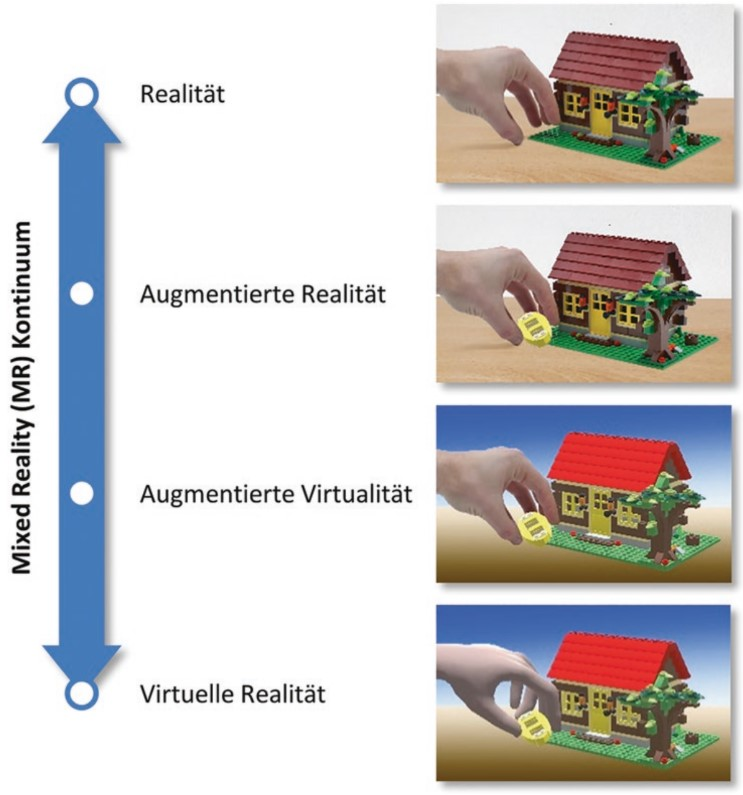
\includegraphics[ width=.5\textwidth ]{Continuum}
    \caption{Kontinuum der Mixed Reality Technologien\label{fig:Continuum}}\par
\end{figure}

Die Ursprünge von AR reichen bis in die 1960er Jahre zurück, als Ivan Sutherland mit seiner Vision des ,,ultimativen Displays'' (\citet{sutherland1965ultimateDisplay}) den Grundstein legte. In seinen Forschungen beschrieb er die Idee einer interaktiven, computergenerierten Welt und verglich sie mit einem ,,Wunderland, wie Alice es betrat''. 

Im Jahr 1968 entwickelte Sutherland gemeinsam mit seinem Studenten Bob Sproull ein \textit{Head-Mounted Display}. Dieses System ermöglichte es Nutzern erstmals, einfache dreidimensionale Formen in der realen Umgebung zu visualisieren. Dabei trägt der Benutzer eine Kopfapparatur, die an der Decke befestigt sind. Das Gerät zeichnet die Rotation des Kopfes auf und überträgt die Bewegungen auf die virtuellen Objekte, die durch die Linsen sichtbar werden. Dies gilt als die erste praktische Anwendung von AR. \cite{sutherland19683dDisplay, doerner2022virtual}

\begin{figure}
    \centering
    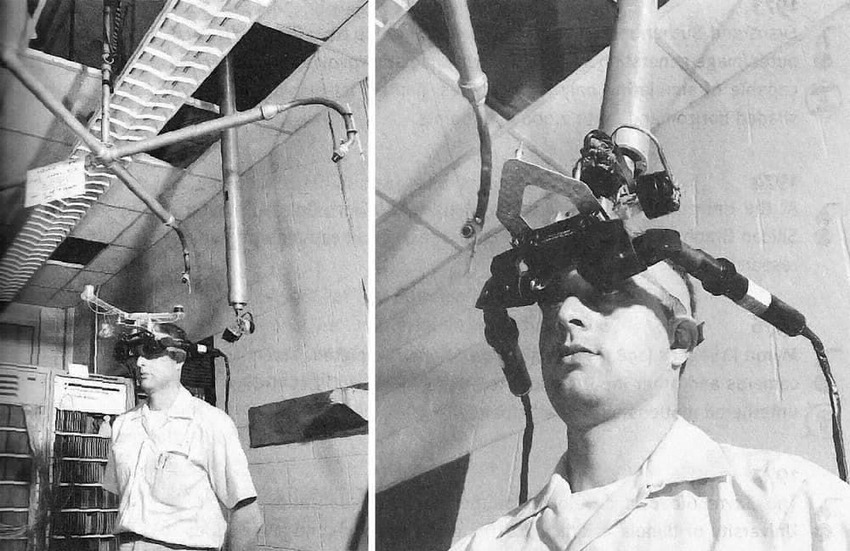
\includegraphics[ width=.5\textwidth ]{HeadMountedDisplay}
    \caption{Sutherlands "Head-Mounted-Display" \cite{sutherland1965ultimateDisplay}\label{fig:HeadMountedDisplay}}\par
\end{figure}

In den folgenden Jahrzehnten wurden zahlreiche technologische Hürden überwunden, die die Entwicklung von AR zuvor behindert hatten. Fortschritte in der Rechenleistung, die Miniaturisierung von Sensoren sowie die kontinuierliche Verbesserung der Bildverarbeitung trugen maßgeblich zur heutigen Leistungsfähigkeit von AR-Anwendungen bei. \cite{doerner2022virtual}

Die Möglichkeiten, digitale Informationen auf interaktive und visuell ansprechende Weise darzustellen, eröffnen ein breites Spektrum an Einsatzgebieten. Dieses Potenzial wurde in verschiedenen Branchen erkannt und in innovativen Anwendungen umgesetzt (siehe Abbildung \ref{fig:MRApplications}). Ein populäres Beispiel ist das mobile Spiel \textit{Pokémon Go} (\citet{wikipedia2024pokemonGo}), bei dem Spieler virtuelle Kreaturen in der realen Welt fangen. In der Medizin dient AR der Visualisierung medizinischer Daten und der Unterstützung bei chirurgischen Eingriffen, wodurch Präzision und Behandlungsergebnisse verbessert werden können (\citet{chen2017medicalMR}).

Auch große Technologieunternehmen haben das Potenzial von AR erkannt: Mit Geräten wie der \textit{Meta Quest 3} und der \textit{Apple Vision Pro} wurde die Technologie erneut in den Fokus der Öffentlichkeit gerückt und eine neue Welle der Begeisterung ausgelöst. \cite{doerner2022virtual, boulanger2024applications}

\begin{figure}[h]
    \centering
    \begin{minipage}{0.45\textwidth}
        \centering
        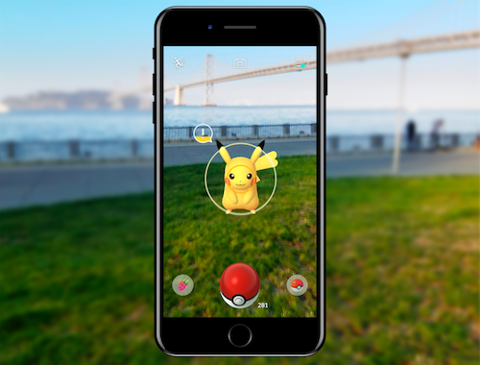
\includegraphics[width=\textwidth]{PokemonGo}
    \end{minipage}
    \begin{minipage}{0.45\textwidth}
        \centering
        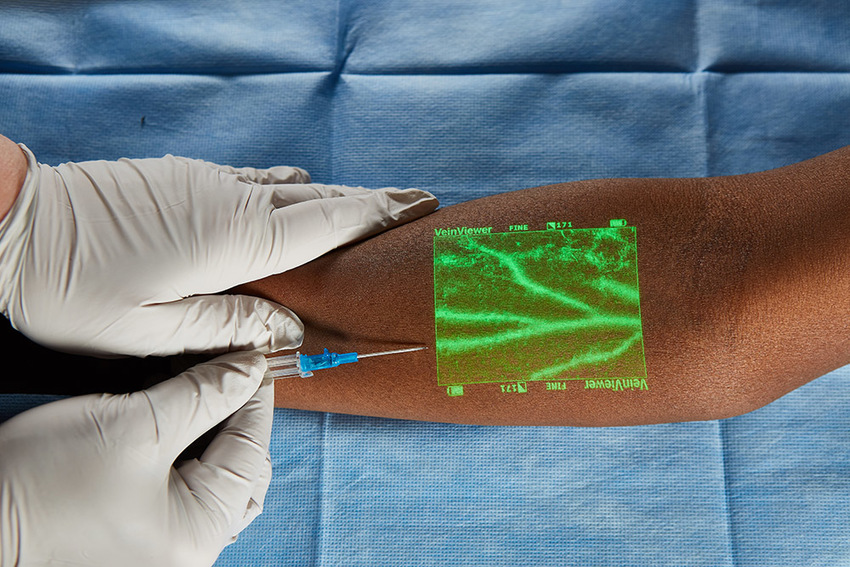
\includegraphics[width=\textwidth]{VeinViewer}
    \end{minipage}
    \begin{minipage}{0.45\textwidth}
        \centering
        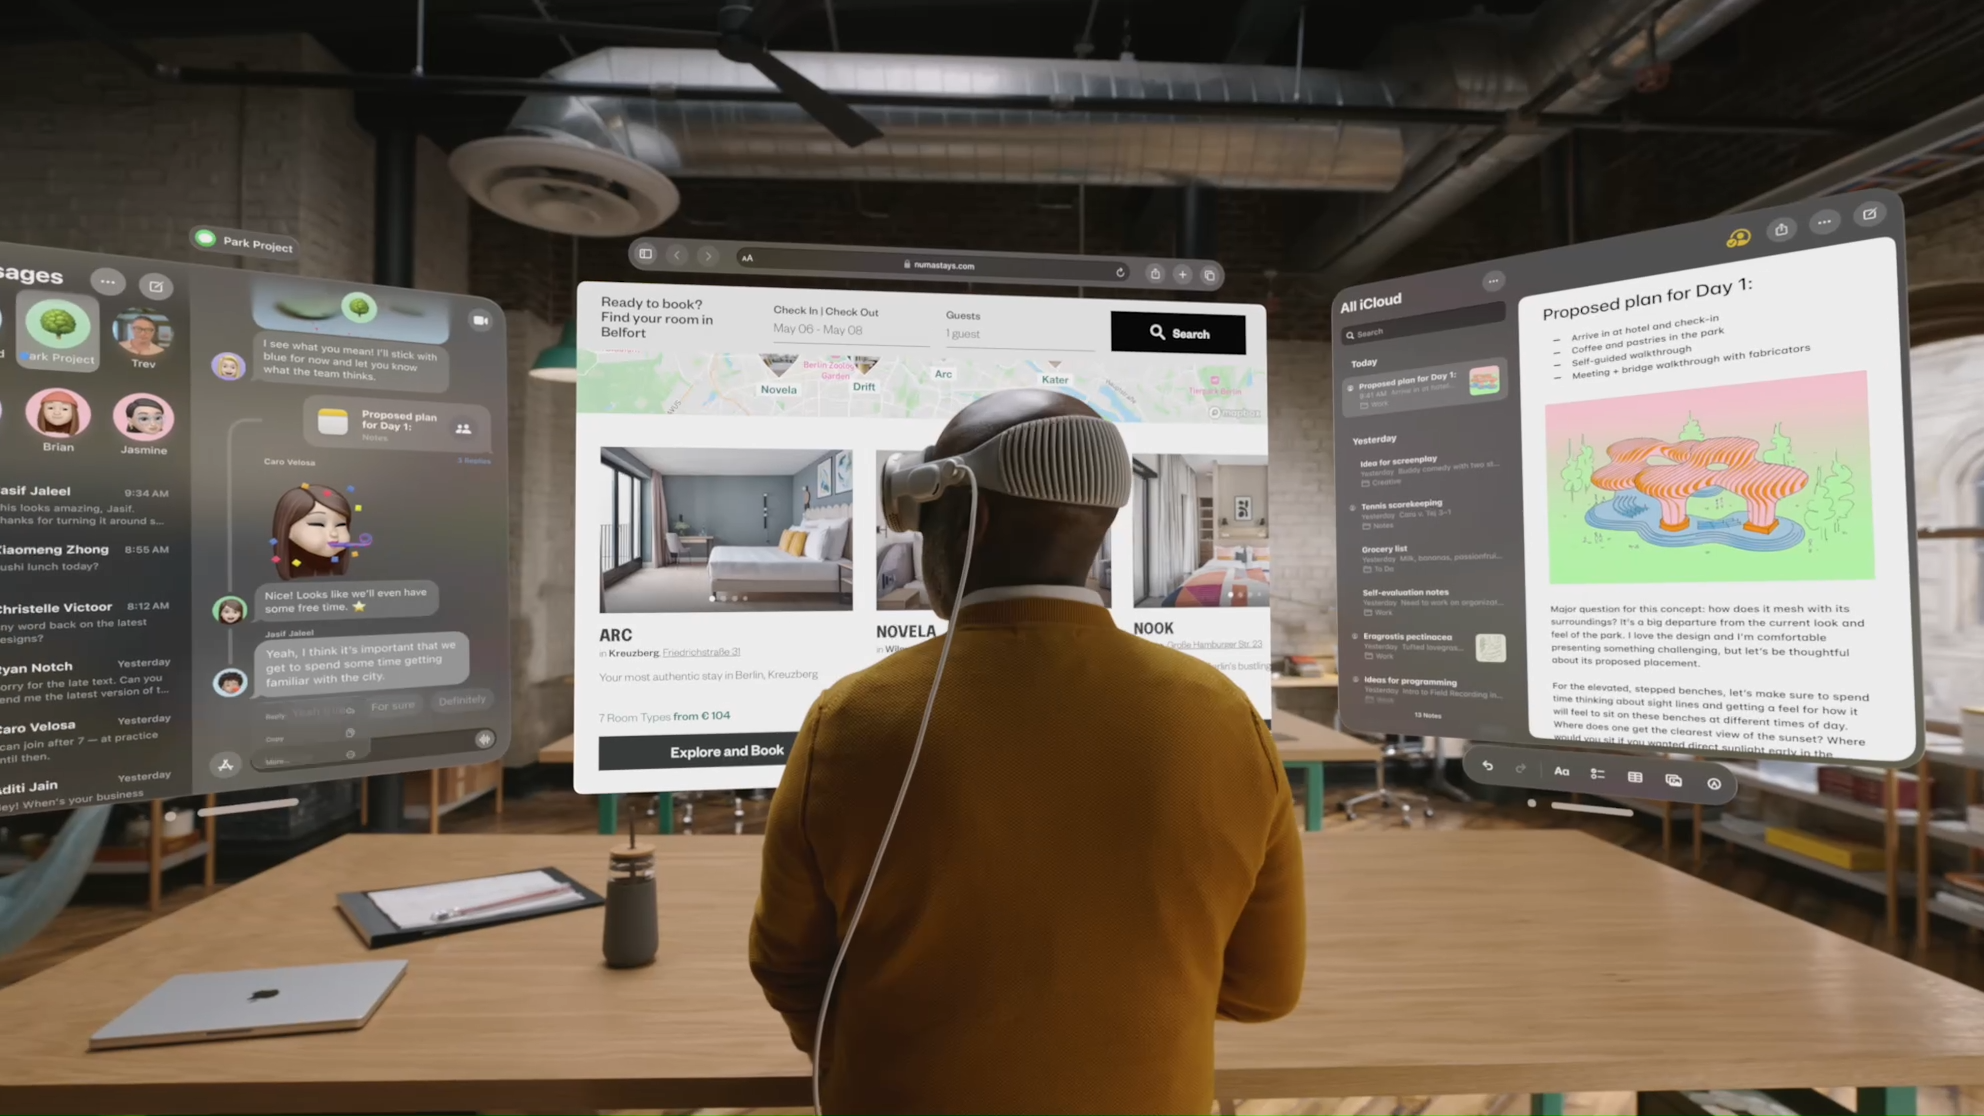
\includegraphics[width=\textwidth]{VisionPro}
    \end{minipage}
    \caption{Beispiele für MR-Anwendungen in verschiedenen Branchen: Pokémon Go (oben links), VeinViewer (oben rechts) und Apple Vision Pro (unten) \cite{wikipedia2024pokemonGo, chen2017medicalMR, apple2023visionPro}}
    \label{fig:MRApplications}
\end{figure}

\section{Zielsetzung}

Ziel dieser Arbeit ist es, das Potenzial von Augmented Reality zur Optimierung von Geschäftsprozessen in einem praxisnahen Anwendungsszenario aufzuzeigen. Bei diesem Szenario handelt es sich um die Montage von Rauchmeldern, einem alltäglichen Prozess in der BRUNATA-METRONA GmbH \& Co. KG.

Dazu sollen die theoretischen Grundlagen von Augmented Reality in Bezug auf die Implementierung einer mobilen Anwendung analysiert und zusammengefasst werden. Dabei werden die mathematischen Konzepte und Algorithmen, die für die Entwicklung von AR-Anwendungen relevant sind, untersucht und erläutert.

Auf Basis dieser Erkenntnisse wird ein Prototyp einer mobilen AR-Anwendung entwickelt, die den Montageprozess visuell unterstützt. Durch den gezielten Einsatz von AR soll der Prozess effizienter und benutzerfreundlicher gestaltet werden. Der Prototyp wird in einer realitätsnahen Umgebung getestet und evaluiert, um die Effektivität der AR-Technologie zu bewerten und mögliche Optimierungspotenziale aufzuzeigen.

Darüber hinaus wird untersucht, inwieweit AR-Technologien nachhaltig in bestehende Arbeitsabläufe integriert werden können. Die langfristigen Auswirkungen auf Produktivität, Schulungsaufwand und Benutzerfreundlichkeit werden kritisch reflektiert.

Die Ergebnisse dieser Arbeit sollen als Entscheidungsgrundlage für den möglichen Einsatz von AR im Montageprozess von Rauchmeldern dienen und eine Basis für zukünftige AR-Projekte bei BRUNATA-METRONA schaffen.

\section{Struktur der Arbeit}

Zu Beginn dieser Arbeit wird die Problemstellung im Kontext der BRUNATA-METRONA GmbH \& Co. KG erläutert. Anschließend wird das methodische Vorgehen bei der Recherche und Ausarbeitung beschrieben. 

Im dritten Kapitel werden die theoretischen Grundlagen von Augmented Reality und die technischen Konzepte, die für die Implementierung einer mobilen AR-Anwendung relevant sind, dargestellt. Dazu gehören mathematische Prinzipien, Tracking- und Rekonstruktionsalgorithmen sowie die Integration von AR.

Im Hauptteil der Arbeit wird die Entwicklung und Implementierung des AR-Prototypen beschrieben. Hierbei werden die Anforderungen an die Anwendung definiert, die technische Umsetzung erläutert und die Implementierung der Montageregeln beschrieben. 

Anschließend wird die Evaluation des Prototypen beschrieben, bei der die Funktionalität und Benutzerfreundlichkeit der Anwendung in einer praxisnahen Umgebung getestet und bewertet werden.

Im letzten Kapitel wird ein Fazit gezogen. Dabei werden die Ergebnisse der Arbeit zusammengefasst und mögliche Erweiterungen und Optimierungen des AR-Prototypen diskutiert.

